\subsection{Aproximación por mínimos cuadrados discretos.}
Considere el problema de calcular los valores de una función en puntos no tabulados, dados los datos experimentales en la siguiente tabla:
\begin{center}
  \begin{tabular}{|c|c|}
    \hline
    $x_i$ & $y_i$\\
    \hline 
    $1$ & $1.3$\\
    $2$ & $3.5$\\
    $3$ & $4.2$\\
    $4$ & $5.0$\\
    $5$ & $7.0$\\
    $6$ & $8.8$\\
    $7$ & $10.1$\\
    $8$ & $12.5$\\
    $9$ & $13.0$\\
    $10$ & $15.6$\\
    \hline
  \end{tabular}
\end{center}
La siguiente figura muestra una gráfica de los valores de la tabla:
\begin{center}
  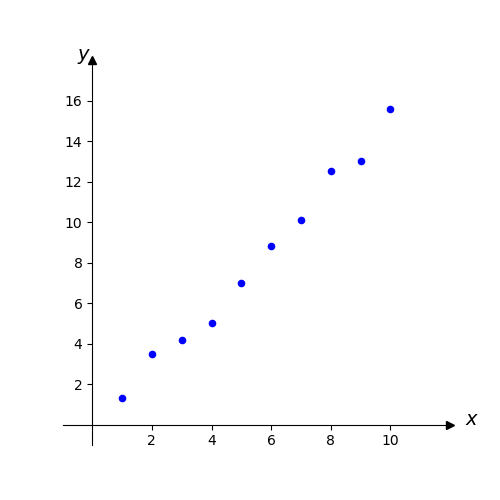
\includegraphics[scale=0.7]{chapters/chapter02/scripts/tabla.png}  
\end{center}
A partir de esta gráfica, parece que la relación real entre $x$ y $y$ es lineal. La razón probable para que ninguna linea se ajuste con precisión a los datos son los errores en estos últimos. Por lo que es poco razonable solicitar que la función de aproximación concuerde exactamente con los datos. De hecho, dicha función introduciría oscilaciones que no estaban presentes originalmente. Por ejemplo, la gráfica del polinomio de interpolación de noveno grado para los datos de la tabla se verán en la siguiente figura:
\begin{center}
  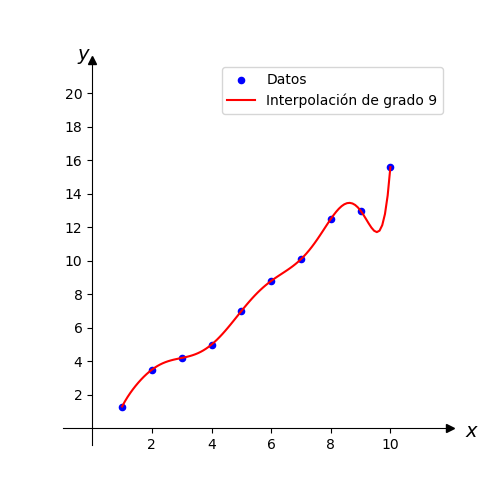
\includegraphics[scale=1]{chapters/chapter02/scripts/tabla-interpolacion.png}
\end{center}
Este polinomio es claramente una predicción de la información entre una serie de puntos de datos. Un mejor enfoque seria encontrar la recta que se aproxima “mejor” (en cierto sentido), incluso si no concuerda precisamente con los datos en ningún punto.\\
Sea que $a_1x_i+a_0$ denota el $i$-ésimo valor en la recta de aproximación y que $y_i$ es el $i$-ésimo valor de $y$ dado. Suponemos que las variables independientes, las $x_i$, son exactas; son las variables dependientes, las $y_i$, de las que sospechamos. Esto es una suposición razonable en muchas situaciones experimentales.\\
El problema de encontrar la ecuación de la mejor aproximación lineal en el sentido
absoluto requiere encontrar los valores $a_0$ y $a_1$ para minimizar:
\begin{align*}
  E_{\infty}(a_0,a_1)=\max_{1\leq i\leq 10}\{y_i-(a_1x_i+a_0)\}.
\end{align*}
Normalmente esto recibe el nombre de problema minimáx y no es posible manejarlo con técnicas fundamentales.\\
Otro enfoque para determinar la mejor aproximación lineal implica encontrar los valores de $a_0$ y $a_1$ para minimizar: 
\begin{align*}
  E_1(a_0,a_1)=\sum_{i=1}^{10}|y_i-(a_1x_i+a_0)|.
\end{align*}
Esta cantidad recibe el nombre de \textbf{desviación absoluta}. Para minimizar una función de dos variables, necesitamos igualar sus derivadas parciales a cero y resolver simultáneamente las ecuaciones resultantes. En el caso de la desviación absoluta, necesitamos encontrar $a_0$ y $a_1$ con:
\begin{align*}
  0=\frac{\partial }{\partial a_0}\sum_{i=1}^{10}|y_i-(a_1x_i+a_0)|\hspace{0.2cm}y\hspace{0.2cm}0=\frac{\partial }{\partial a_1}\sum_{i=1}^{10}|y_i-(a_1x_i+a_0)|.
\end{align*}
El problema es que la función valor absoluto no es diferenciable en cero y podríamos no encontrar soluciones para este par de ecuaciones.
\subsubsection{Mínimos cuadrados lineales.}
  El enfoque de mínimos cuadrados para este problema implica determinar la mejor linea de aproximación cuando el error relacionado es la suma de los cuadrados de las diferencias entre los valores $y$ en la linea de aproximación y los valores $y$ proporcionados. Por lo tanto, deben encontrarse las constantes $a_0$ y $a_1$ que minimizan el error de mínimos cuadrados:
  \begin{align*}
    E_2(a_1,a_0)=\sum_{i=1}^{10}[y_i-(a_1x_i+a_0)]^2.
  \end{align*}
  El método de mínimos cuadrados es el procedimiento mas conveniente para determinar mejores aproximaciones lineales, pero también hay consideraciones técnicas importantes que lo favorecen. En general, mientras el enfoque minimáx asigna demasiado peso a un bit de datos con un gran error, el método de desviación absoluta no da suficiente peso a un punto que esté fuera de la linea con la aproximación. El enfoque de mínimos cuadrados asigna considerablemente mas peso en un punto que esta fuera de la linea que al resto de los datos, pero no permitir que el punto domine por completo la aproximación. Una razón adicional para considerar el enfoque de mínimos cuadrados implica el estudio de la distribución estadística del error. 
  El problema general de ajustar la mejor linea de mínimos cuadrados para una recopilación de datos $\{x_i,y_i\}_{i=1}^{m}$, implica minimizar el error total,
  \begin{align*}
    E\equiv E_{2}(a_0,a_1)=\sum_{i=1}^{m}[y_i-(a_1x_i+a_0)]^{2},
  \end{align*}
  respecto a los parámetros $a_0$ y $a_1$. Para que se presente un mínimo, necesitamos que:
  \begin{align*}
    \frac{\partial E}{\partial a_0}=0\hspace{0.2cm}y\hspace{0.2cm}\frac{\partial E}{\partial a_1}=0,
  \end{align*}
  es decir,
  \begin{align*}
    0=-2\sum_{i=1}^{m}(y_i-a_1x_i-a_0)
  \end{align*}
  y
  \begin{align*}
    0=-2\sum_{i=1}^{m}(y_i-a_1x_i-a_0)(x_i)
  \end{align*}
  Estas ecuaciones zzz
